\section{Quadcopter flight tests}

After validating the performance of the control algorithms in the simulated environment, the next step involves conducting flight tests with a fully built physical UAV. This final phase of the validation process aims to assess the performance of the developed software with all the previously analysed components together in a real quadcopter during flight. To achieve this, first, the base vehicle will be constructed using the chosen development kit. Subsequently, all additional components required for this project, such as the companion computer and camera, will be integrated into the base frame. The developed control solutions will be tested once the vehicle can successfully fly with the entire payload under remote control.

The initial test will run the hand-control solution to verify that the autopilot can receive flight commands from an offboard computer outside the simulation. Next, the follow mechanism will be started to confirm that the companion computer can function in flight as well as it did during the simulation tests. The exact steps that will be executed one after the other to ensure that safety is guaranteed during the whole process are as follows:
\begin{enumerate}
    \item Assemble the quadcopter with the custom payload.
    \item Baseline flight with factory software. Conduct a test flight using only the remote control and factory autopilot while monitoring through QGroundControl.
    \item Offboard computer flight with \texttt{test-camera} tool. Perform a flight controlled by the DroneVisionControl software running on an offboard computer (laptop).
    \item Onboard computer flight with \texttt{test-camera} tool. Conduct a flight controlled by the DroneVisionControl software running on the onboard computer (Raspberry Pi).
    \item Hand-gesture control with offboard computer. Control the drone with hand gestures by running the hand-gesture control solution on the offboard computer.
    \item Follow control with onboard computer. The drone flies following a target person by running the follow control solution on the onboard computer.
\end{enumerate}


\subsection{Build process}
\label{sec:test-7-builddrone}

The chosen vehicle for this project is the Holybro X500, specifically designed to be compatible with PX4. The PX4 documentation\footnote{\url{https://docs.px4.io/main/en/frames_multicopter/holybro_x500_pixhawk4.html}} provides detailed instructions on how to build the vehicle using its Development Kit. Figure \ref{fig:x500-dev-kit} illustrates all the components required to construct the complete vehicle.

\begin{figure}[H]
  \centering
  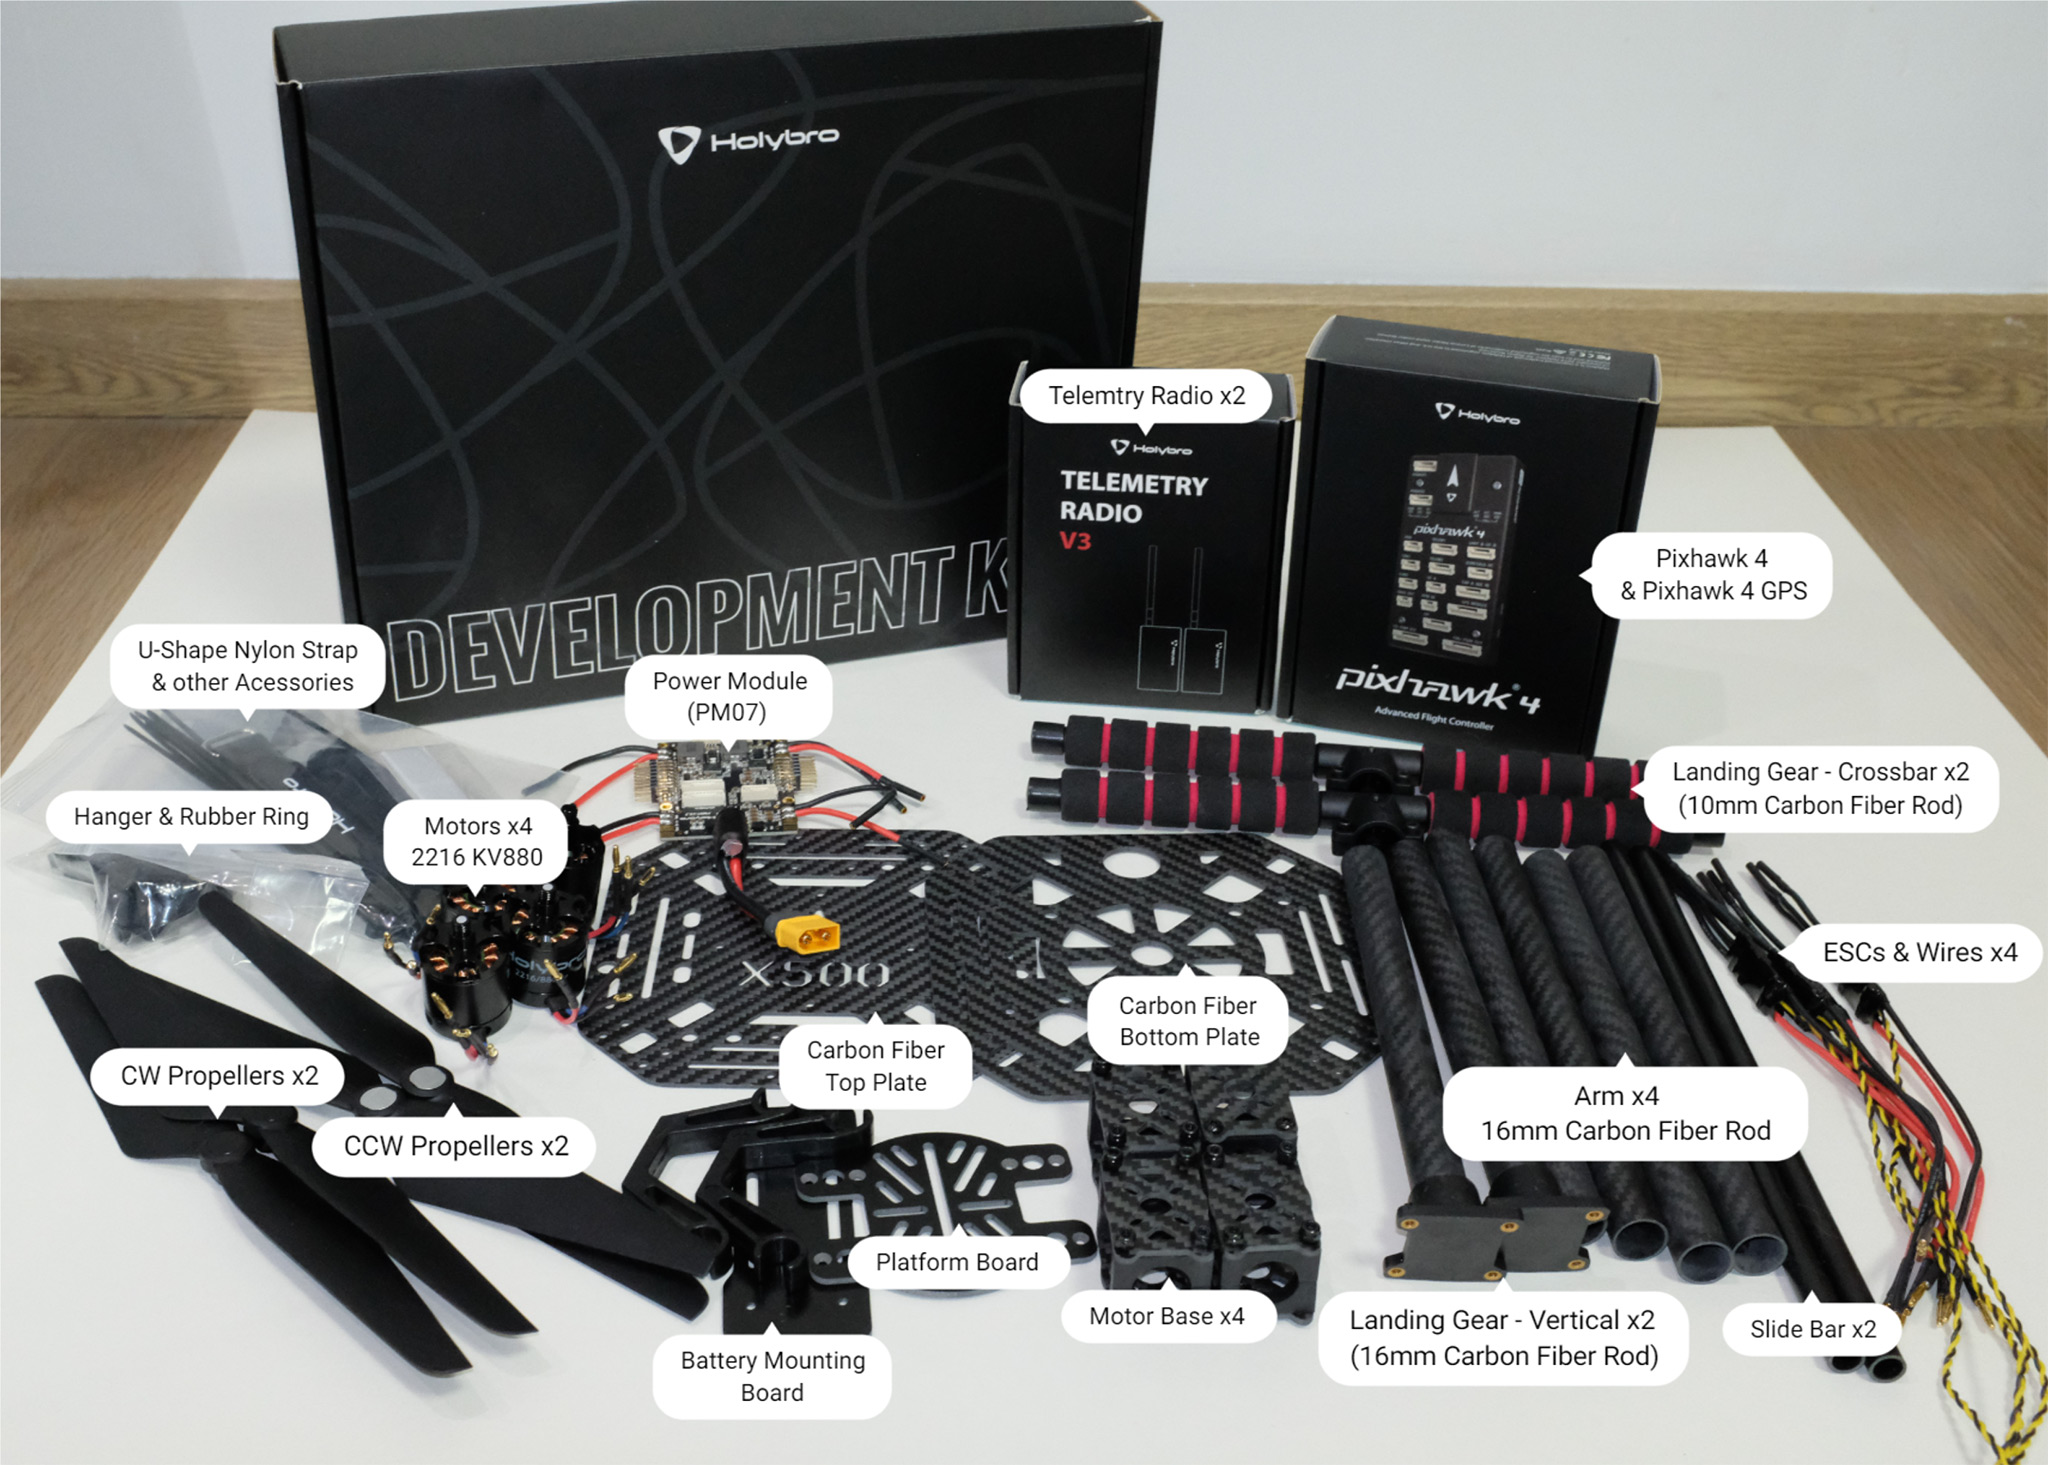
\includegraphics[width=.9\textwidth, keepaspectratio]{img/x500-dev-kit.jpg}
  \caption{Development kit for the Holybro X500.}
  \source{Adapted from \citetitle{px4-guide} \cite{px4-guide}.}
  \label{fig:x500-dev-kit}
\end{figure}


Once the standard parts are assembled, the custom additions can be integrated into the remaining space within the frame. The Raspberry Pi companion computer will be positioned between the autopilot and GPS antenna (see Figure \ref{fig:full-build}). This placement facilitates a convenient connection between the autopilot and the Raspberry Pi's I/O pins using short cables, preventing excessive wire clutter within the frame. During flight, the Raspberry Pi will be powered by a dedicated external battery, separate from the main battery powering the motors, which supplies power through a 2-ampere USB port. This port will be connected to the Raspberry Pi's USB-C power supply socket with a charging cable. As explained in Section \ref{sec:test-5-rpi}, the power supply by this secondary battery is sufficient to operate the connected camera and run the developed software with satisfactory performance. The battery will be positioned beneath the autopilot, as depicted in Figure \ref{fig:full-build}. 


\begin{figure}[H]
  \centering
  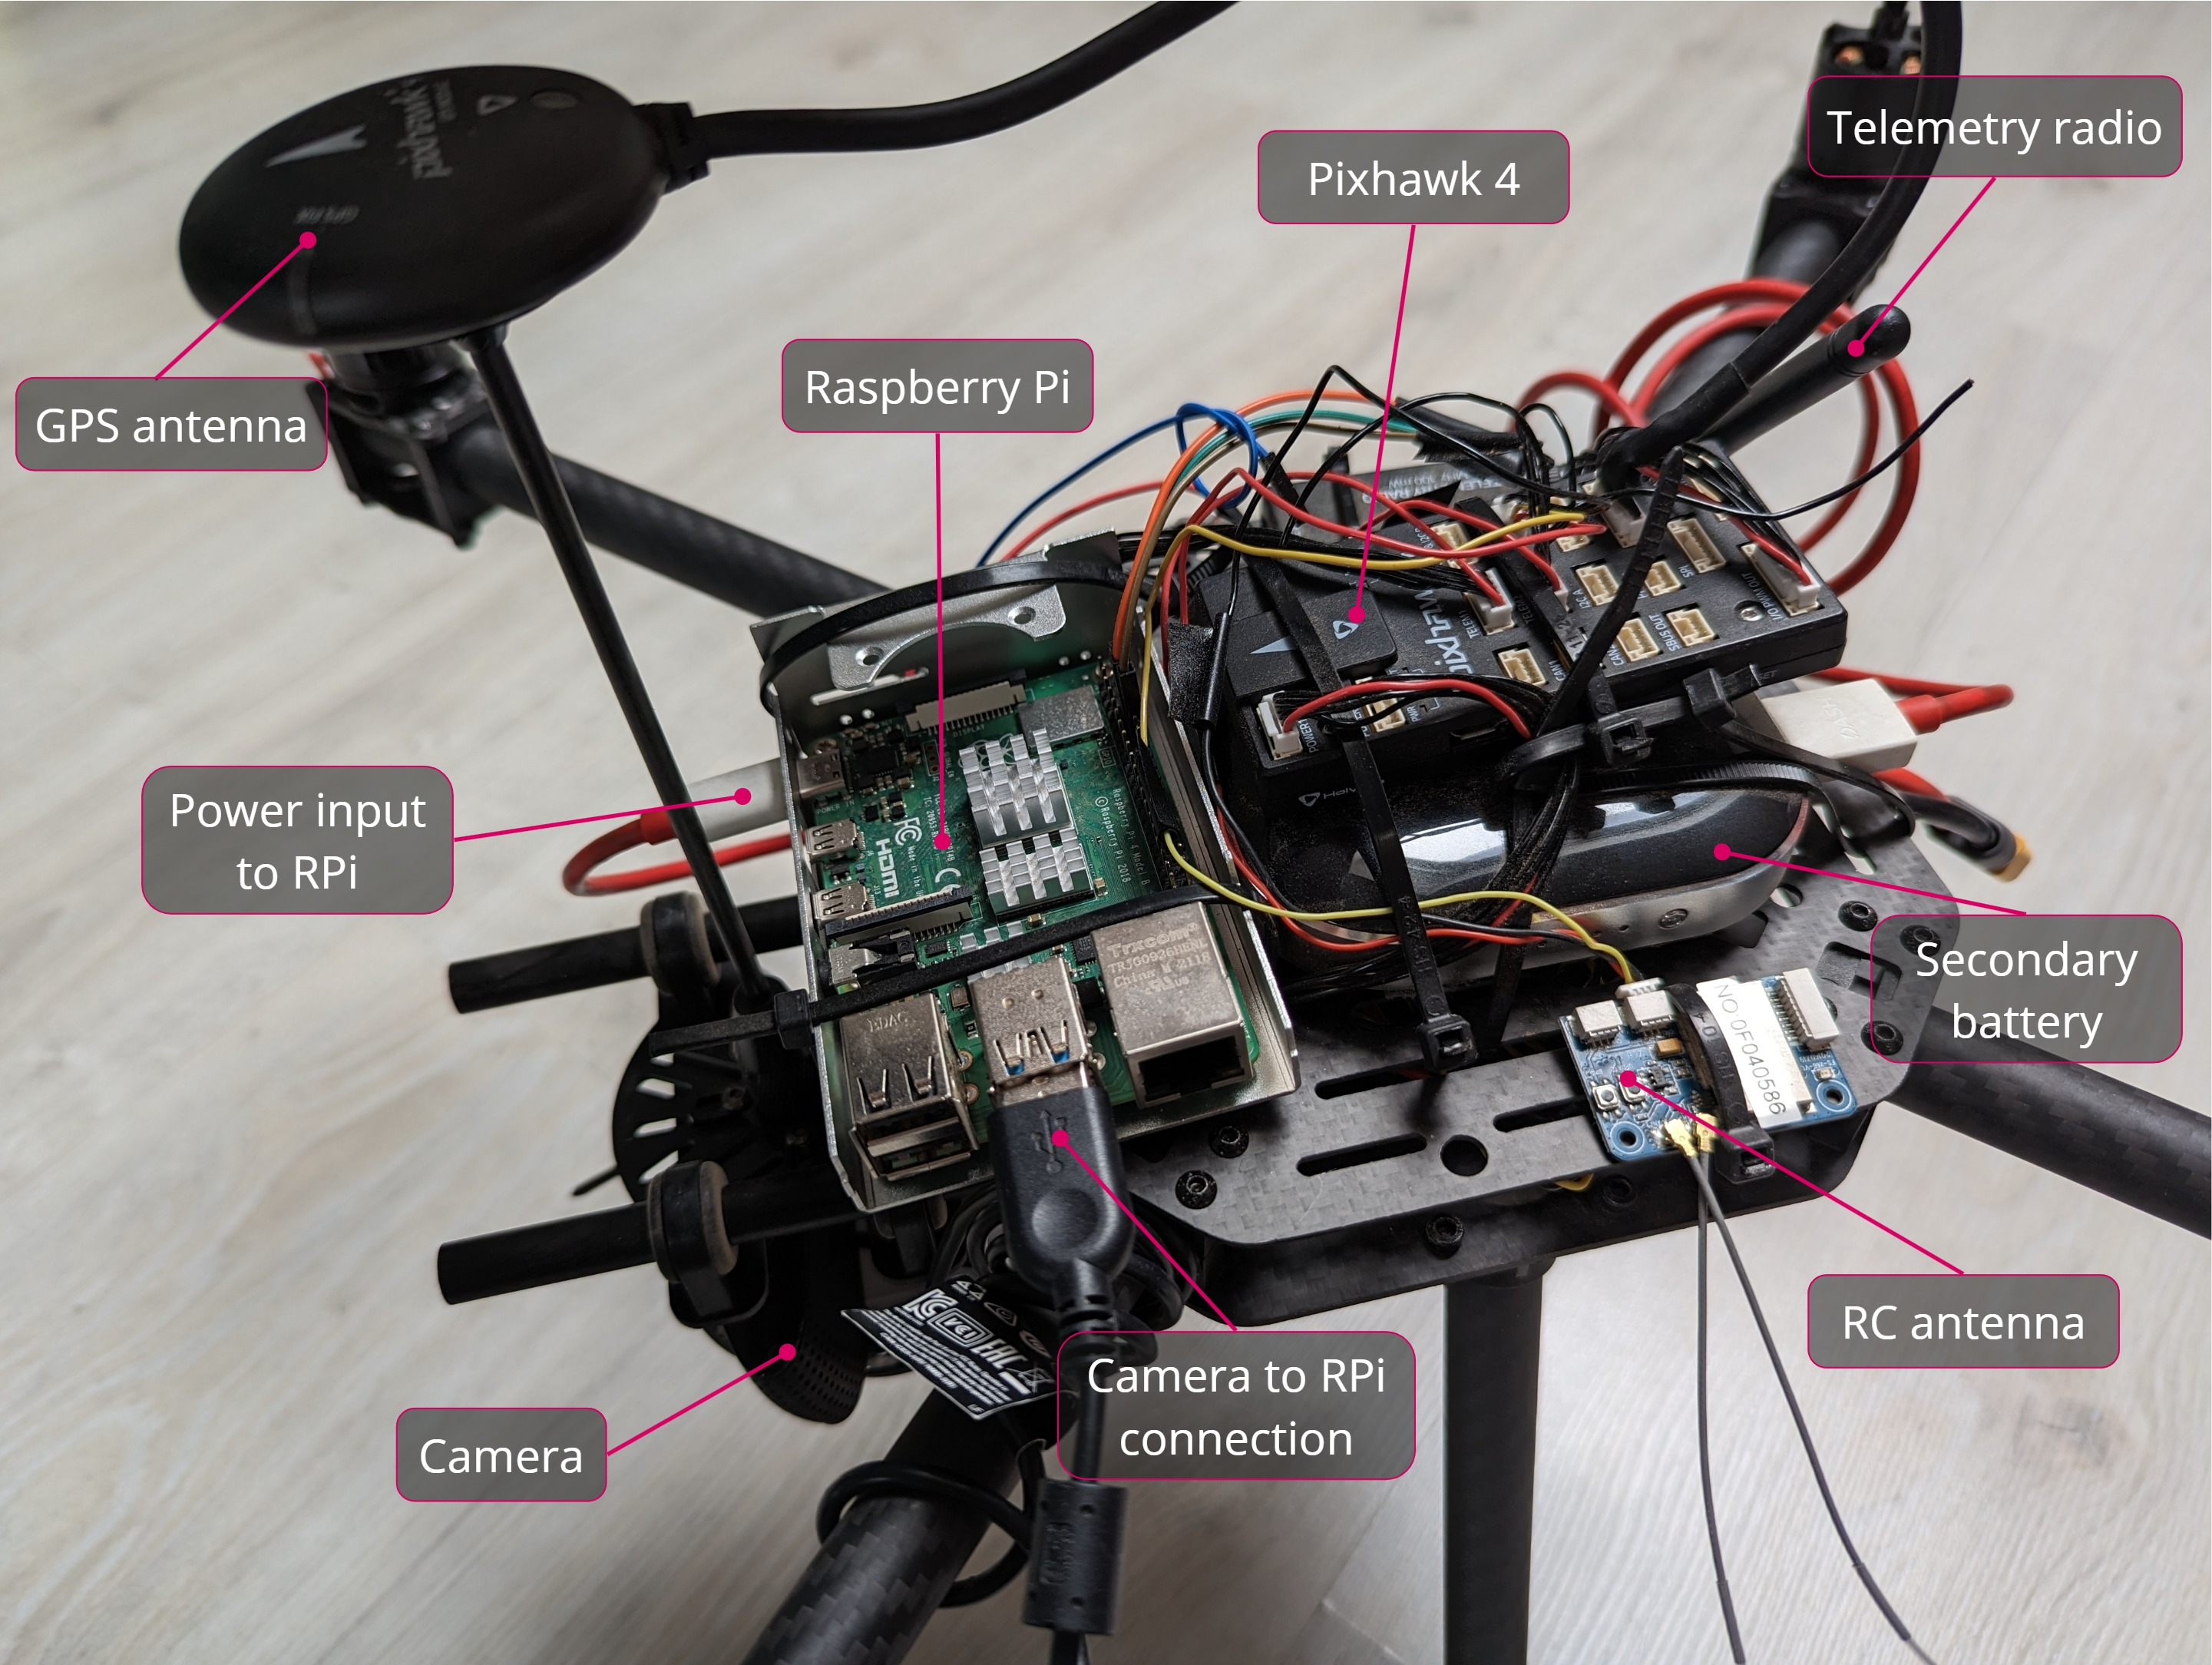
\includegraphics[width=1\textwidth, keepaspectratio]{img/full-build.jpg}
  \caption{Complete build of the quadcopter with the main components highlighted.}\label{fig:full-build}
\end{figure}


To ensure the camera is securely mounted on the vehicle's frame, the custom-built support system described in Section \ref{subsec:onboard} will be utilized. The camera holder will be attached to the slide bars beneath the main frame, positioning the camera's weight as close to the centre of mass as possible behind the GPS platform (see Figure \ref{fig:camera-holder-closeup}). The main battery, responsible for powering the engines and autopilot, and located on the underside of the carbon frame, can be shifted along the forward axis to balance the added weight from the companion computer, its battery and the camera so that the centre of gravity falls approximately in the centre of the vehicle.

\begin{figure}[H]
  \centering
  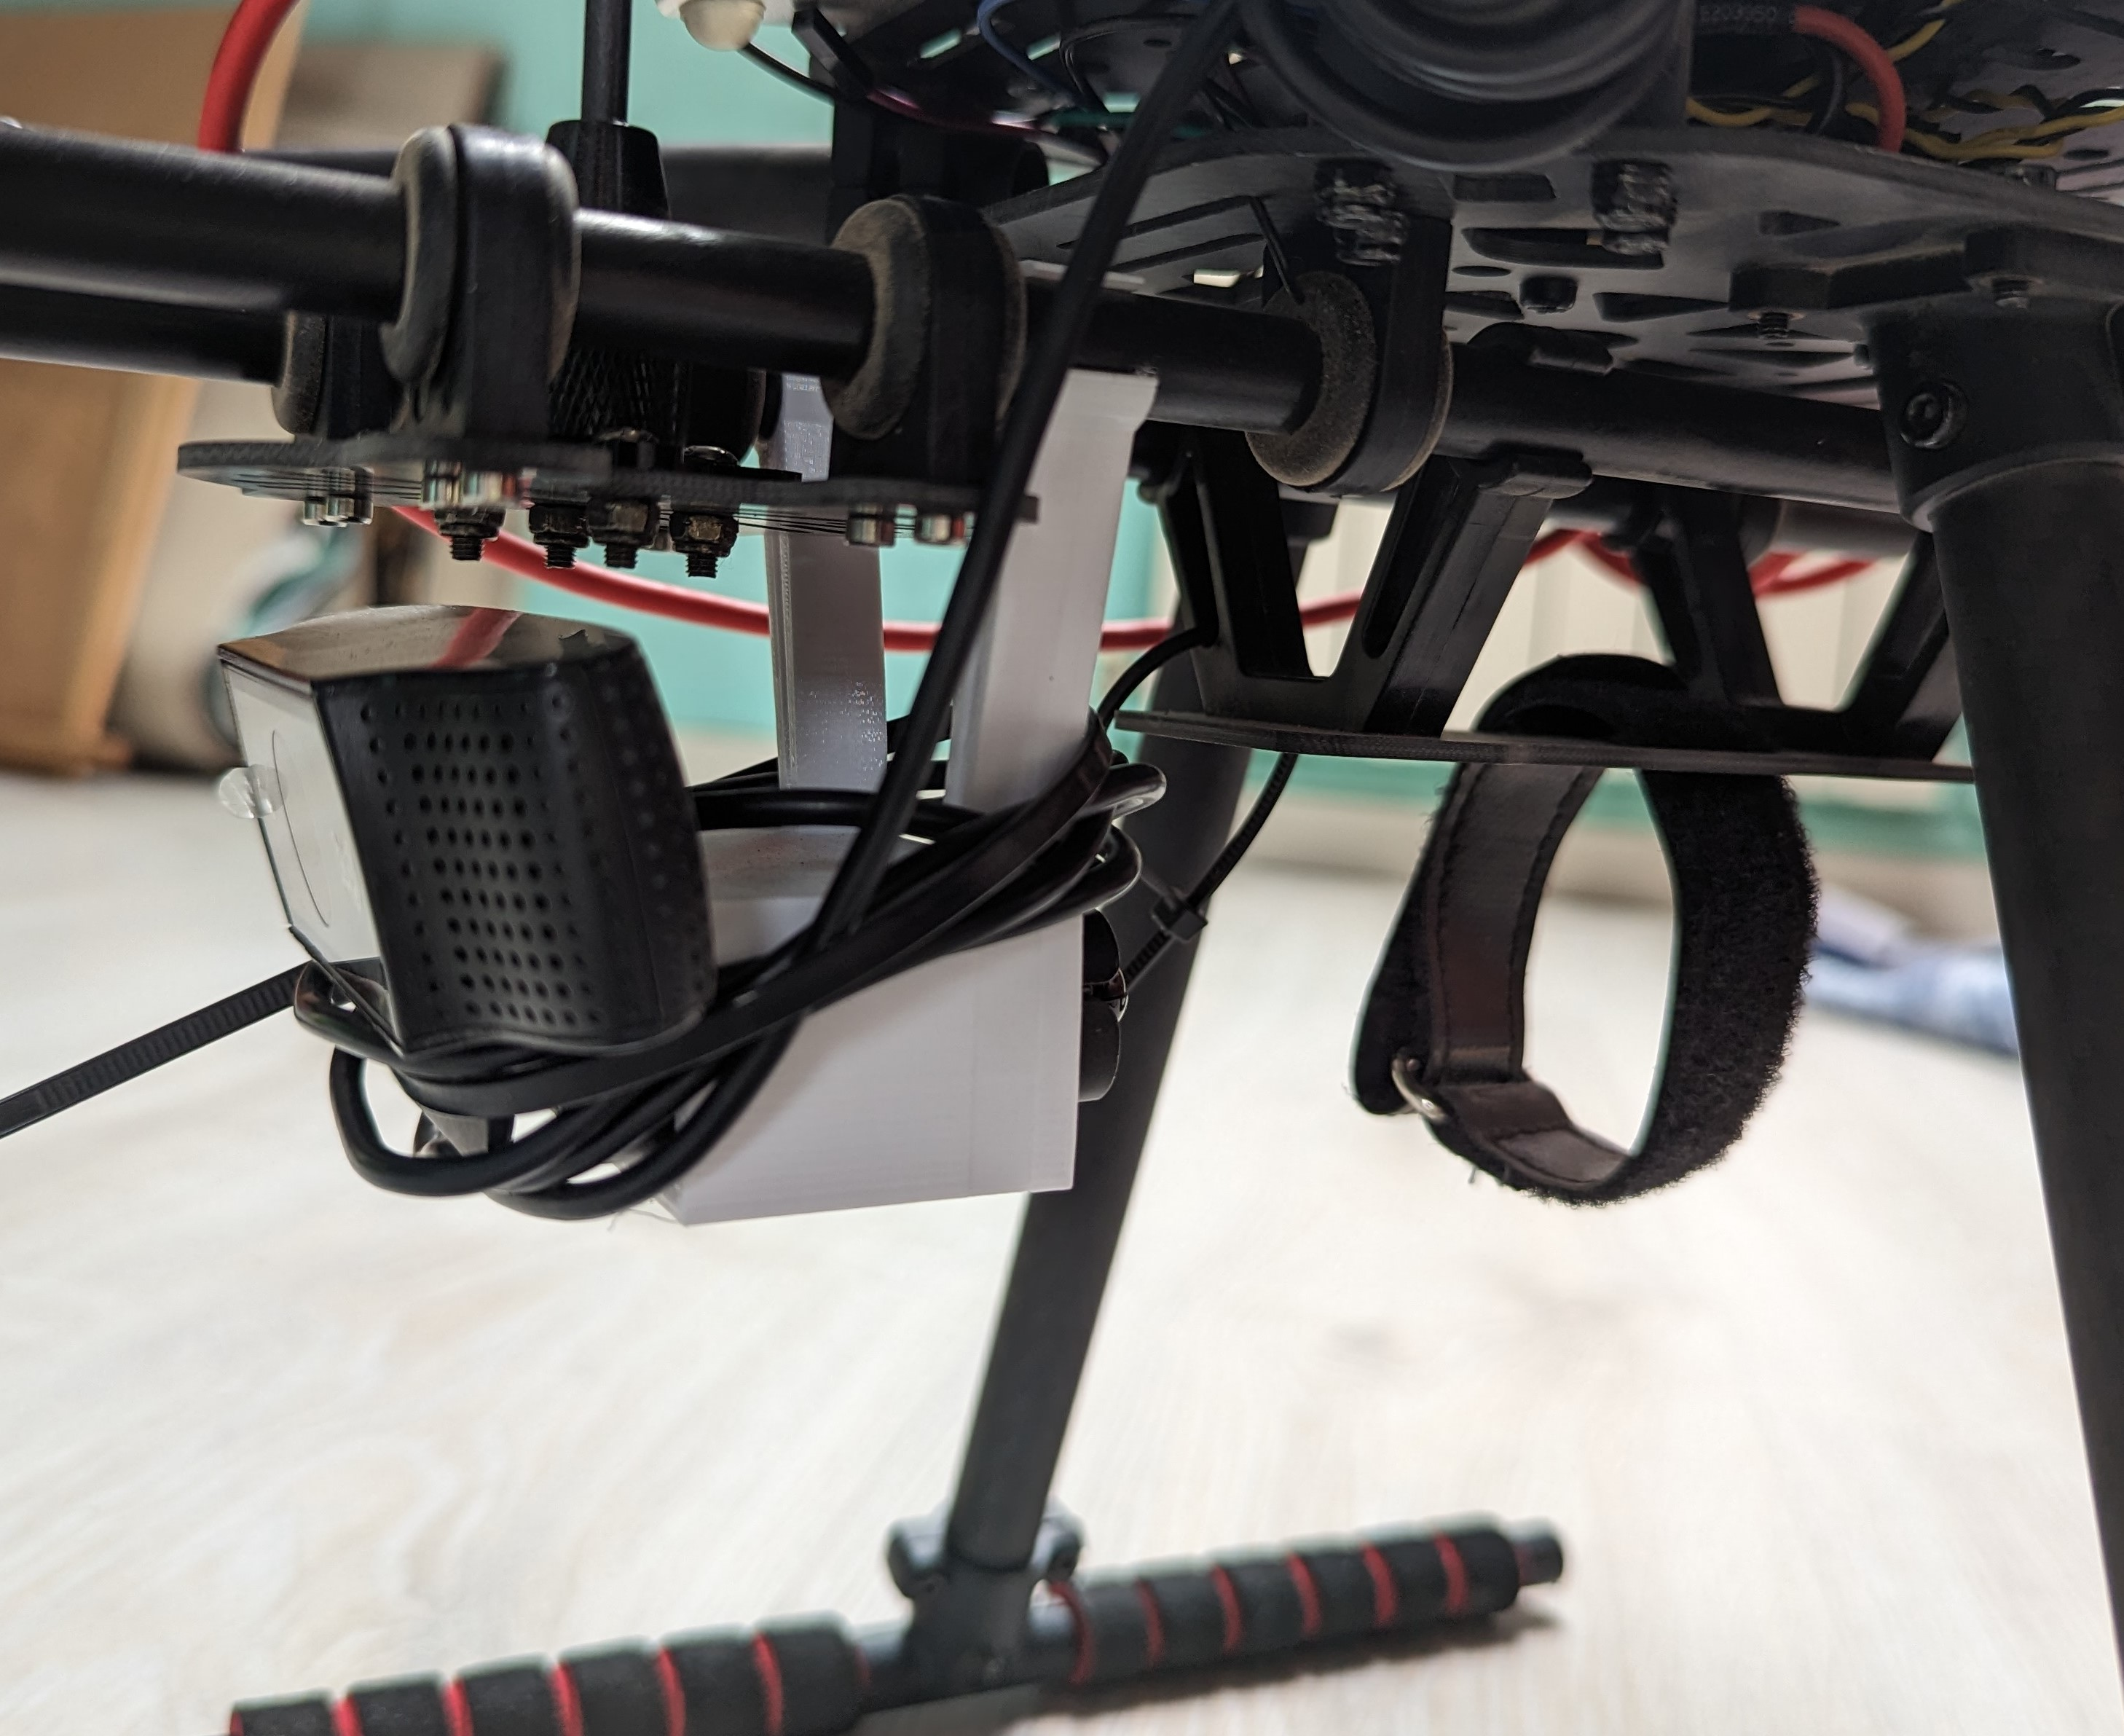
\includegraphics[width=0.75\textwidth, keepaspectratio]{img/underside-2.jpg}
  \caption{Underside of the vehicle, with the supports for holding the main battery and the camera in place.}
  \label{fig:camera-holder-closeup}
\end{figure}


Once the vehicle is constructed, additional installation and calibration steps are necessary before it can be flown. This configuration can be performed through QGroundControl by connecting the flight controller to a computer either directly via its debug micro-USB port or wirelessly via the telemetry radio.
The calibration steps are outlined in the Holybro X500 build instructions and are required to ensure that all the sensors attached to the autopilot function correctly. The QGroundControl configuration screens shown in Figure \ref{fig:qgc-config} depict some of these steps. Besides the standard calibration, two additional PX4 settings must be set in the Pixhawk board for the DroneVisionControl software to work. First, the HITL simulation mode needs to be disabled in the QGroundControl safety settings and, second, the \texttt{TELEM2} port should be enabled to communicate with the Raspberry Pi, as explained in Section \ref{subsec:offboard}.


\begin{figure}[H]
  \centering
  \makebox[\textwidth][c]{
  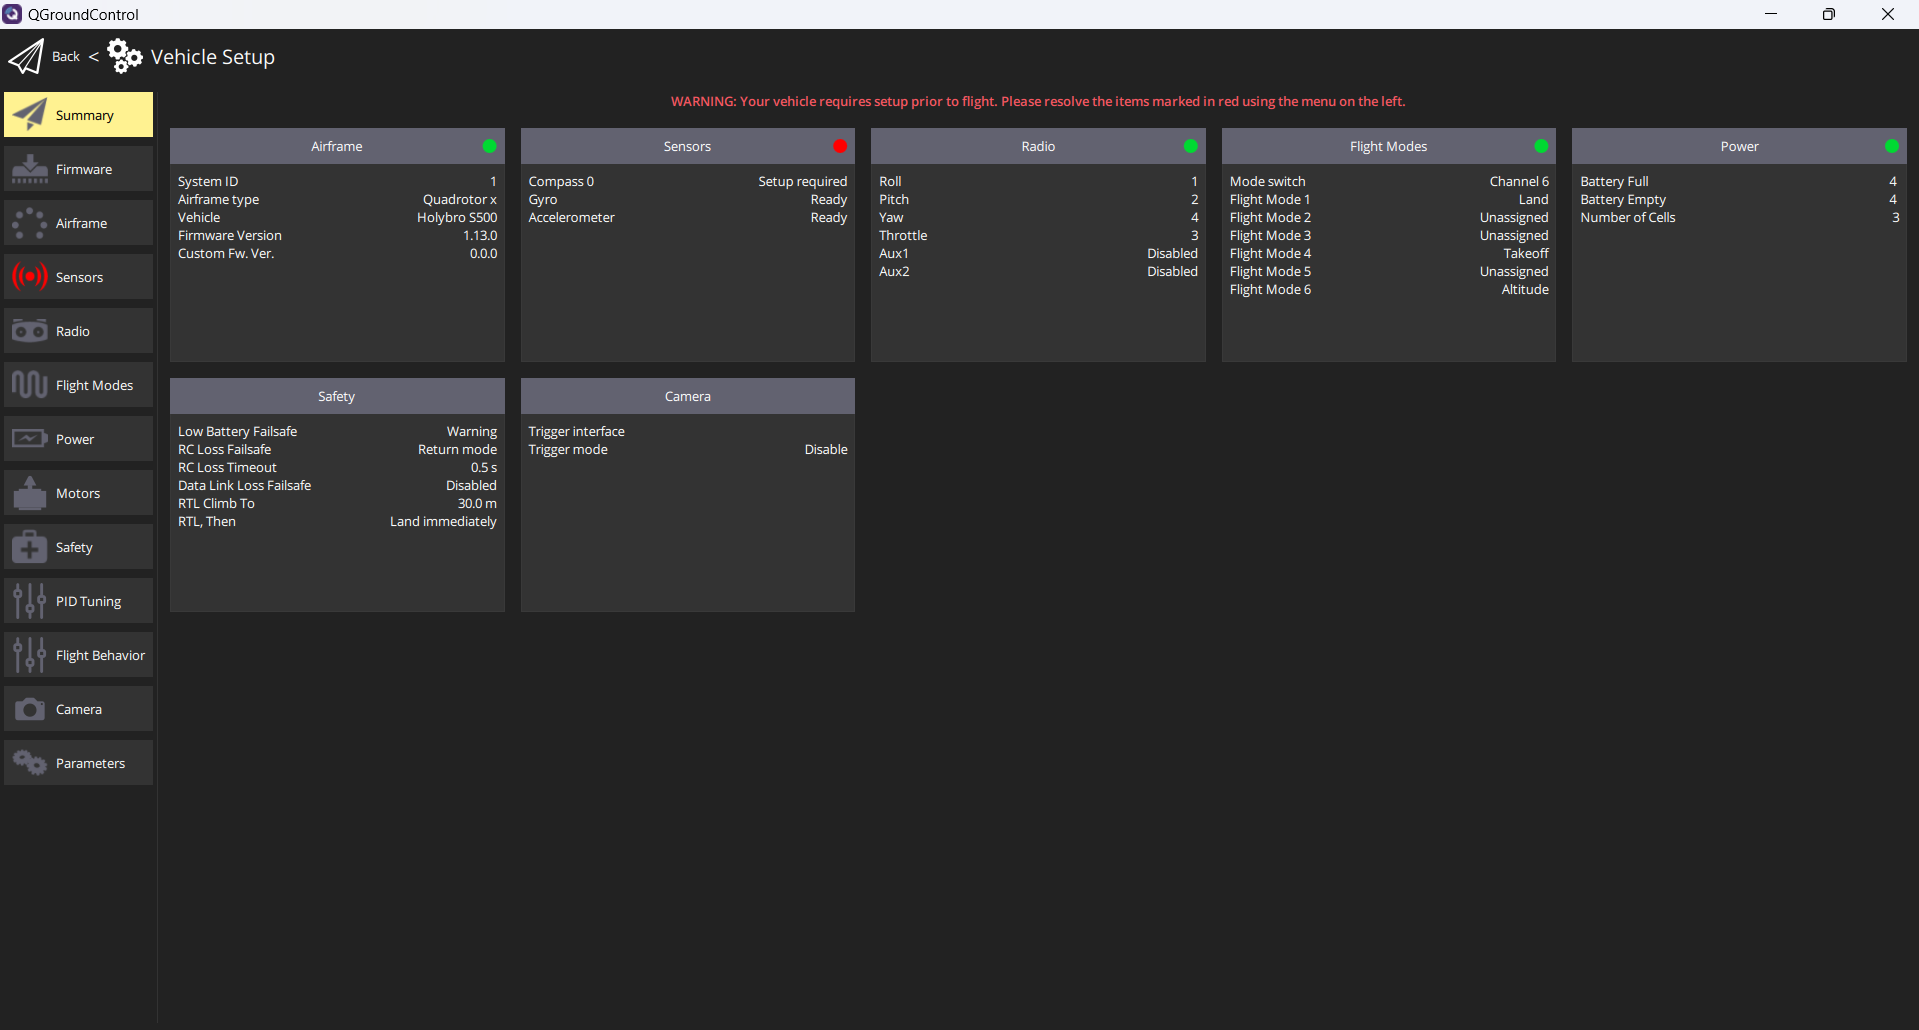
\includegraphics[width=0.5\textwidth, keepaspectratio]{img/qgc-config-1.png}
  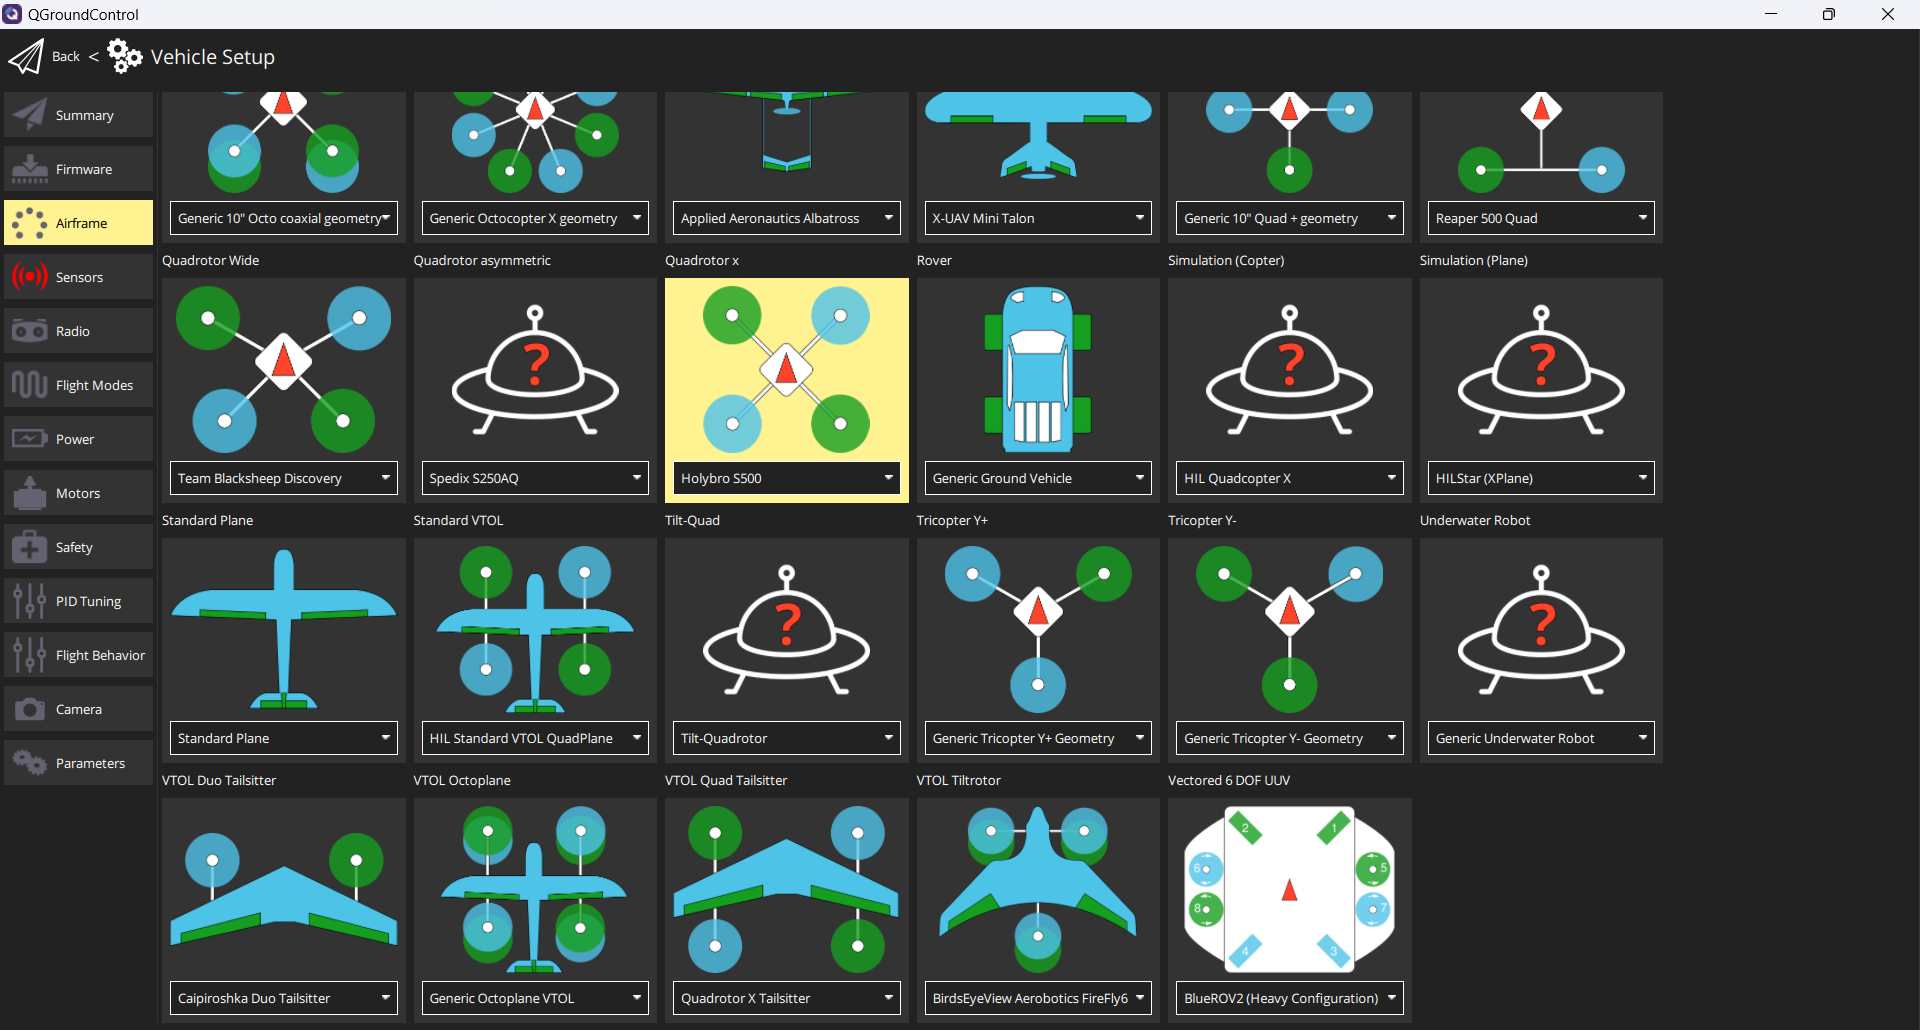
\includegraphics[width=0.5\textwidth, keepaspectratio]{img/qgc-config-3.png}}\\
  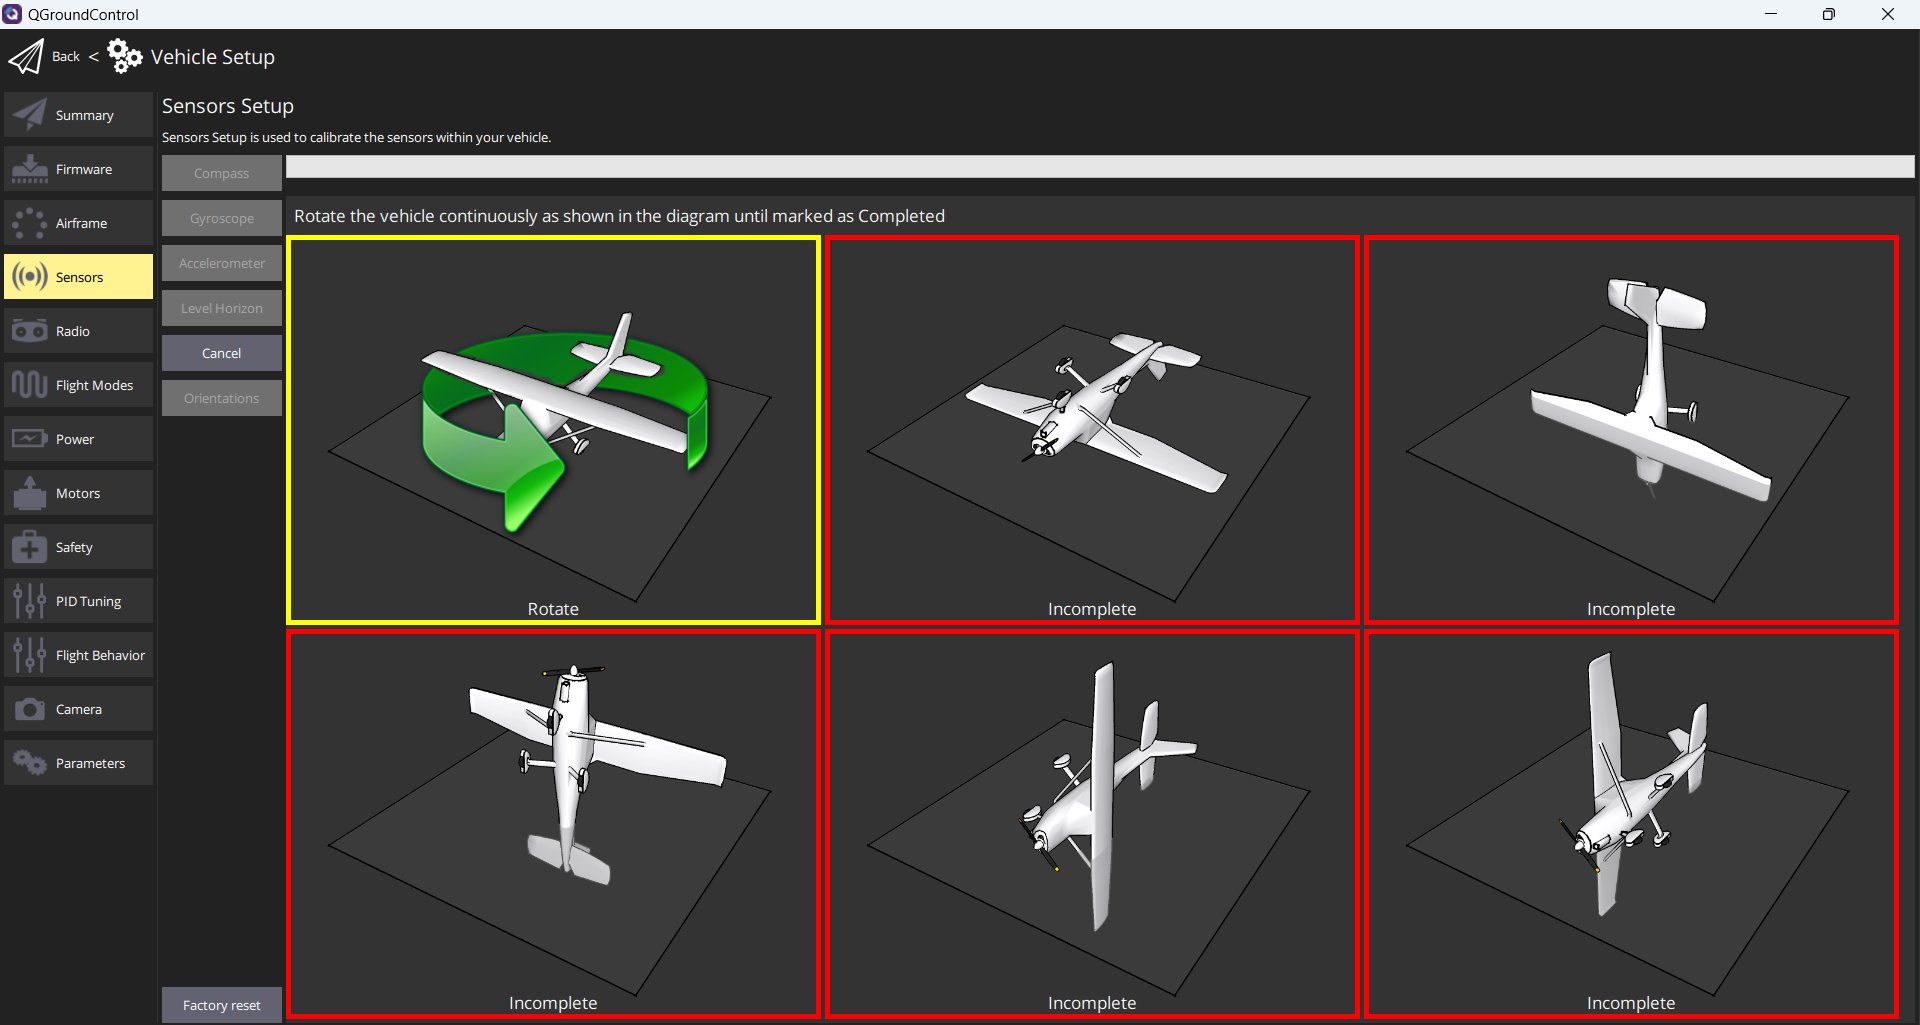
\includegraphics[width=0.5\textwidth, keepaspectratio]{img/qgc-config-2.png}
  \caption{Screenshots from the QGroundControl calibration and setup tools used to configure the vehicle. From the top left: a) overview screen of the state of the vehicle components, a warning indicates that some sensors must be calibrated; b) airframe selection screen; c) gyroscope calibration screen detailing the process.}
  \label{fig:qgc-config}
\end{figure}


\subsection{Initial tests}
\label{sec:test-8-flight}


\subsubsection{Baseline flight with factory software}
\label{subsec:fl-test-1}

Once the vehicle is fully configured and calibrated, testing the assisted takeoff and landing can be conducted using the RC controller and QGroundControl. At this stage, the drone should be capable of maintaining stable flight using autopilot-assisted flight modes, such as Position Mode. In Position Mode, the roll and pitch sticks in the controller control the vehicle's acceleration over the ground in the forward/backward and left/right directions, respectively, relative to the vehicle's heading. The throttle stick controls the ascent and descent speed. When the sticks are centred, the vehicle actively maintains its position in 3D space, compensating for wind and external forces. This semi-manual mode can serve as a safe means to verify the functionality of the factory autopilot.


Through QGroundControl, it is possible to map different switches on the RC controller to various autopilot commands. For the test, a two-position switch will be mapped to the armed/disarmed state in order to control the quadcopter's engine startup. A three-position switch will be assigned to change the vehicle's flight mode between the landing, takeoff and position modes. By shifting between the available switch positions during flight, the primary autopilot modes can be tested. Any other flight modes or triggers that need to be used can be activated directly through the QGroundControl interface during flight.

\todo[inline]{Add picture of RC controller with labels for controls}


To initiate the flight, the main battery is connected to the power module socket. This action powers up the autopilot, GPS antenna, telemetry radio, and RC receiver. Subsequently, QGroundControl is launched on a computer connected to the second telemetry radio via USB. If all connections have been established correctly, the ground station application will automatically connect to the vehicle and display its position on a satellite map. Similarly, turning on the RC controller establishes its connection with the vehicle, provided they have been correctly paired together as outlined in the build instructions guide. Once all wireless connections are established, the drone can take off by switching to the armed state, followed by selecting the takeoff flight mode. While the drone is airborne, switching to the position flight mode enables direct control through the joysticks on the controller.


\subsubsection{Offboard computer flight with test tool}
\label{subsec:fl-test-2}

The second test flight aims to verify that the custom software (DroneVisionControl) can wirelessly transmit takeoff and landing commands from a laptop used as an offboard computer. The MAVLink channel between the autopilot and the computer will be established through the telemetry radio by the developed \texttt{test-camera} tool. It is important to note that, during the flight, the QGroundControl application must be disconnected, as only one application can use the telemetry radio at a time. Consequently, the RC controller will serve as the backup control mechanism in case of any issues with the software. 

The controller can be used to switch flight modes and override inputs from the DroneVisionControl application, providing manual control if necessary in the same way as in the previous test. Since the DroneVisionControl application automatically arms the vehicle when sending a takeoff command, the two-position switch can be repurposed as a kill switch for all subsequent tests. This allows the operator to cut all power to the engines to protect the vehicle or the surrounding area if the autopilot were to malfunction. Some cases when this command can be useful include the vehicle trying to take off sideways because of a poorly balanced payload or a person getting too close to the propellers when the engines are running.

To initiate the test, the main battery is reconnected to the power module. Then, the following command is executed on the offboard computer, depending on whether it is desired to be run on a Windows or Linux machine.


\begin{minted}[escapeinside=||,breaklines,fontsize=\footnotesize, baselinestretch=1]{bash}
|Windows:| dronevisioncontrol tools test-camera --hardware COM<X>:57600
|Linux:| dronevisioncontrol tools test-camera --hardware /dev/ttyUSB0:57600}
\end{minted}


After successfully establishing the connection with the vehicle, the computer keyboard can be used to control the flight to test sending commands from DroneVisionControl. Pressing the T key triggers takeoff, while the L key initiates the landing process. The O key sets the autopilot to offboard flight mode, enabling it to receive velocity commands. These are sent with the WASD keys to control the forward and sideways movement of the vehicle and the QE keys to adjust its yaw rotation. At any point during the test, any input from the RC controller will activate manual control, and the drone will stop listening to the control application.

Figure \ref{fig:flight-test-cam-offboard} illustrates the output displayed in the computer's terminal window, showcasing the connection process, the sent velocity commands, and the camera output from the offboard computer. Additionally, a video capturing the entire process can be accessed in the project's \href{https://l-gonz.github.io/tfg-giaa-dronecontrol/videos/flight-test-offboard}{website}\footnote{\url{https://l-gonz.github.io/tfg-giaa-dronecontrol/videos/flight-test-offboard}}.

\begin{figure}
  \centering
  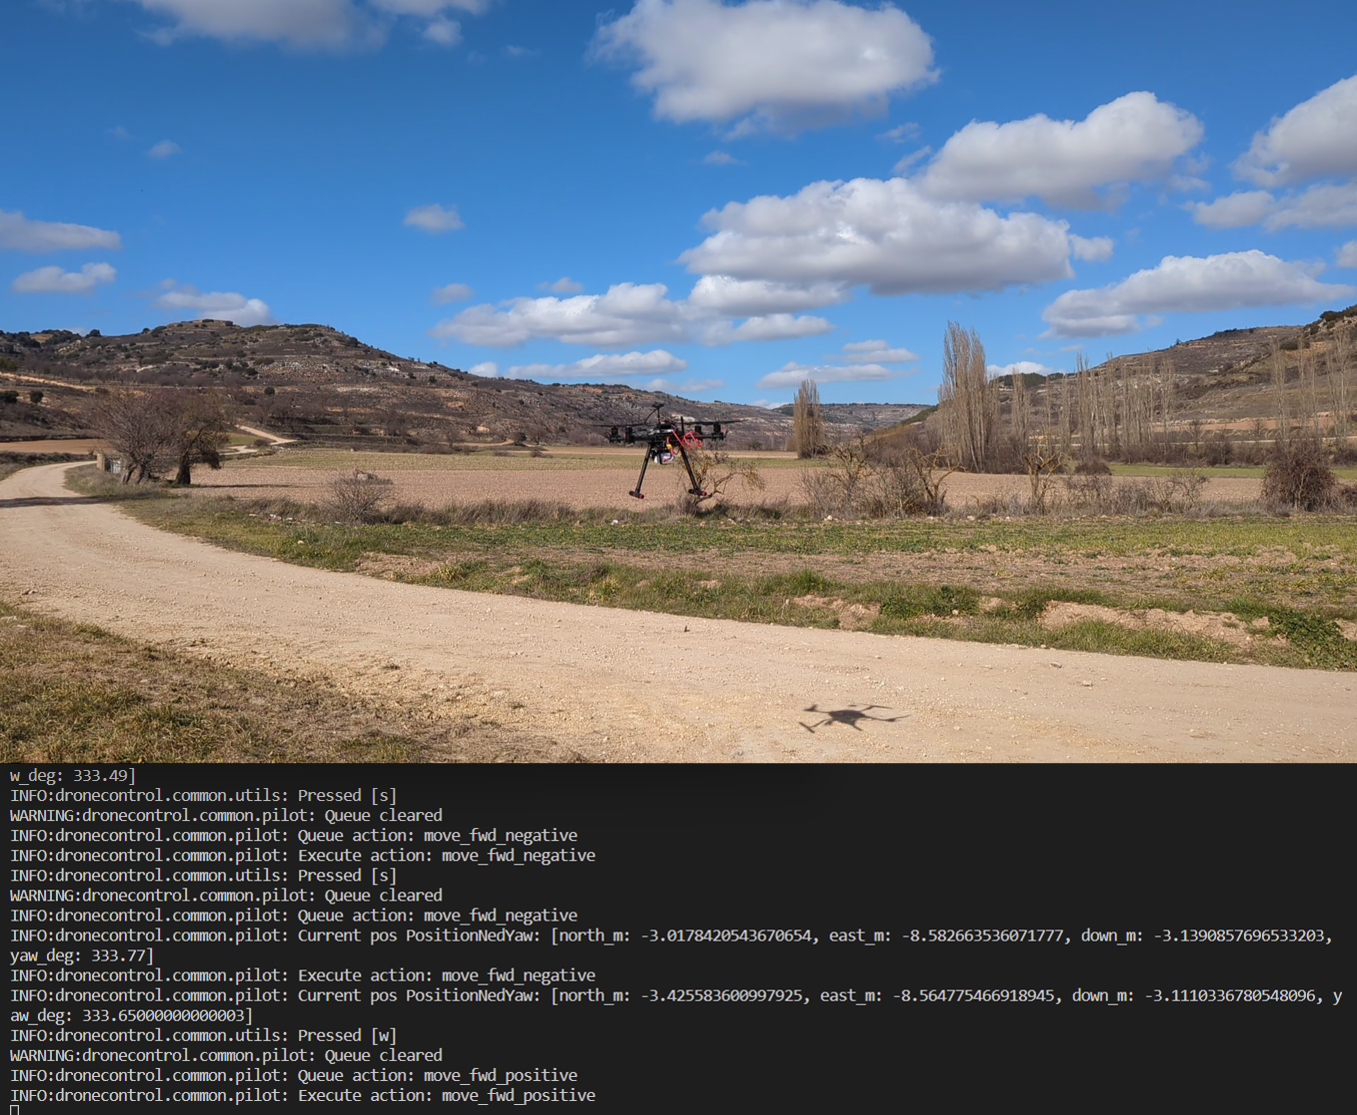
\includegraphics[width=\textwidth, keepaspectratio]{img/video-field-test-offboard.png}
  \caption{Terminal output from the \texttt{test-camera} tool running on an offboard computer and image of the drone flying in response.}
  \label{fig:flight-test-cam-offboard}
\end{figure}

\subsubsection{Onboard computer flight with test tool}
\label{subsec:fl-test-3}


The third and final test flight in this section aims to confirm that the custom software can send takeoff and landing commands through the cabled MAVlink channel to the autopilot from the onboard computer (Raspberry Pi). Additionally, it ensures that the onboard camera can capture images during flight that are clear enough for the pose detection software to detect and track a person in its field of view.

For this test, the same tool used in the previous test will be executed on the Raspberry Pi mounted onboard the vehicle. As the tool will now use the camera connected to the companion computer, positioned to look down on the pilot, pose detection can be activated on the received images.

To initiate the flight test, the main battery is attached to the power module and the secondary battery to the Raspberry Pi. Once the onboard computer has powered up, it can be operated through a remote desktop connection via WiFi. Using this connection, a console can be opened on the Raspberry's desktop to execute the following command:
\begin{minted}[breaklines, fontsize=\footnotesize, baselinestretch=1]{bash}
dronevisioncontrol tools test-camera --hardware /dev/serial0:921600 -p
\end{minted}


Unlike the telemetry radio flight, this test employs a serial connection running at a baud rate of 921600, matching the configured baud rate on the \texttt{TELEM2} port of the Pixhawk board. The \texttt{-p} option enables pose detection in the output images. A video documenting the entire process can be accessed on this \href{https://l-gonz.github.io/tfg-giaa-dronecontrol/videos/flight-test-onboard}{link}\footnote{\url{https://l-gonz.github.io/tfg-giaa-dronecontrol/videos/flight-test-onboard}}. Figure \ref{fig:flight-test-cam-onboard} shows the Raspberry Pi's desktop with pose detection running on the images taken from onboard the vehicle, as transmitted to the ground station laptop via WiFi.


\begin{figure}
  \centering
  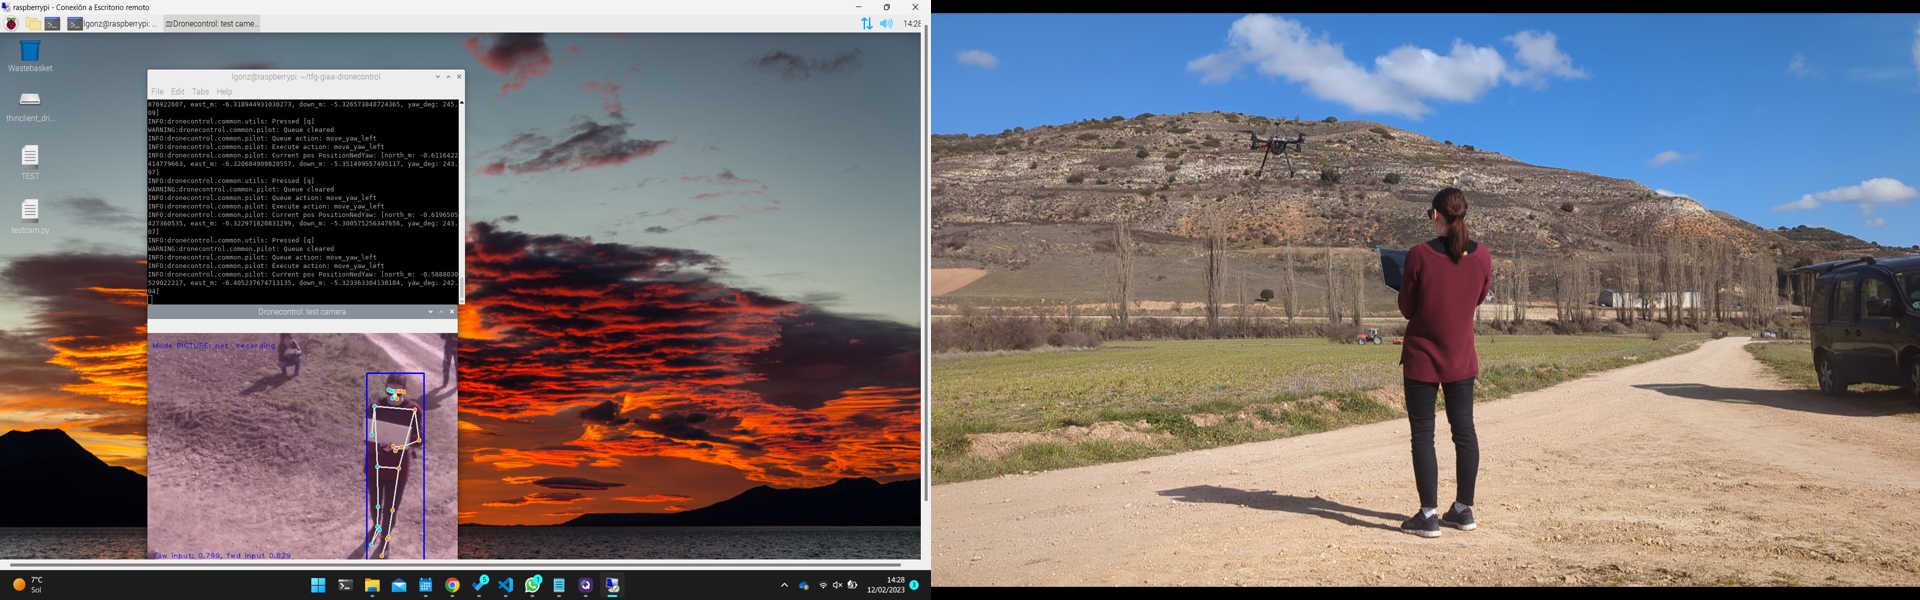
\includegraphics[width=\textwidth, keepaspectratio]{img/video-field-test-onboard.png}
  \caption{On the left, the onboard computer controlled from the ground station laptop runs pose detection while flying. On the right, the drone and the detected person are seen from a different angle}
  \label{fig:flight-test-cam-onboard}
\end{figure}


\subsection{Hand gesture control with offboard computer}
\label{subsec:fl-test-4}


During the basic flight tests, all the connections and individual components of the software were validated in realistic flight scenarios. Now, the focus shifts to integrating the piloting system with the results of image recognition to test the developed vision-based control solutions.

The first solution to be tested in flight is the hand-gesture guidance system, which runs on an offboard computer without performance constraints and doesn't rely on battery power. The setup for this test will be the same as the second test flight, described in Section \ref{subsec:fl-test-2}, using the telemetry radio for the serial link and disregarding the onboard companion computer. Once the autopilot board is powered up, the control solution is initiated by executing the following command, where <device> is replaced with the appropriate COM port or TTY device to which the telemetry radio is connected, depending on the OS of the offboard computer.
\begin{minted}[breaklines, fontsize=\footnotesize, baselinestretch=1]{bash}
dronevisioncontrol hand --serial <device>:57600
\end{minted}


Once the pilot connection is established, the image from the computer's webcam will be displayed on the screen with an outline highlighting any detected hand. The open palm gesture (hold command) can be shown to the camera to test that the hand is correctly recognised without triggering any action. Closing the hand into a fist will initiate takeoff, and pointing up with the index finger will activate the offboard flight mode. Moving the index finger right or left will cause the vehicle to mirror the movement, while moving the thumb right or left will make the vehicle move forward and backward, respectively. At any point during the test, displaying an open hand will cause the drone to hover in its current position. Losing sight of the controlling hand will also trigger the hovering mode.


A video showcasing the entire process can be accessed on this \href{https://l-gonz.github.io/tfg-giaa-dronecontrol/videos/flight-test-hand}{link}\footnote{\url{https://l-gonz.github.io/tfg-giaa-dronecontrol/videos/flight-test-hand}}. Additionally, an image extracted from the video can be seen in Figure \ref{fig:flight-test-hand}.

\begin{figure}[H]
  \centering
  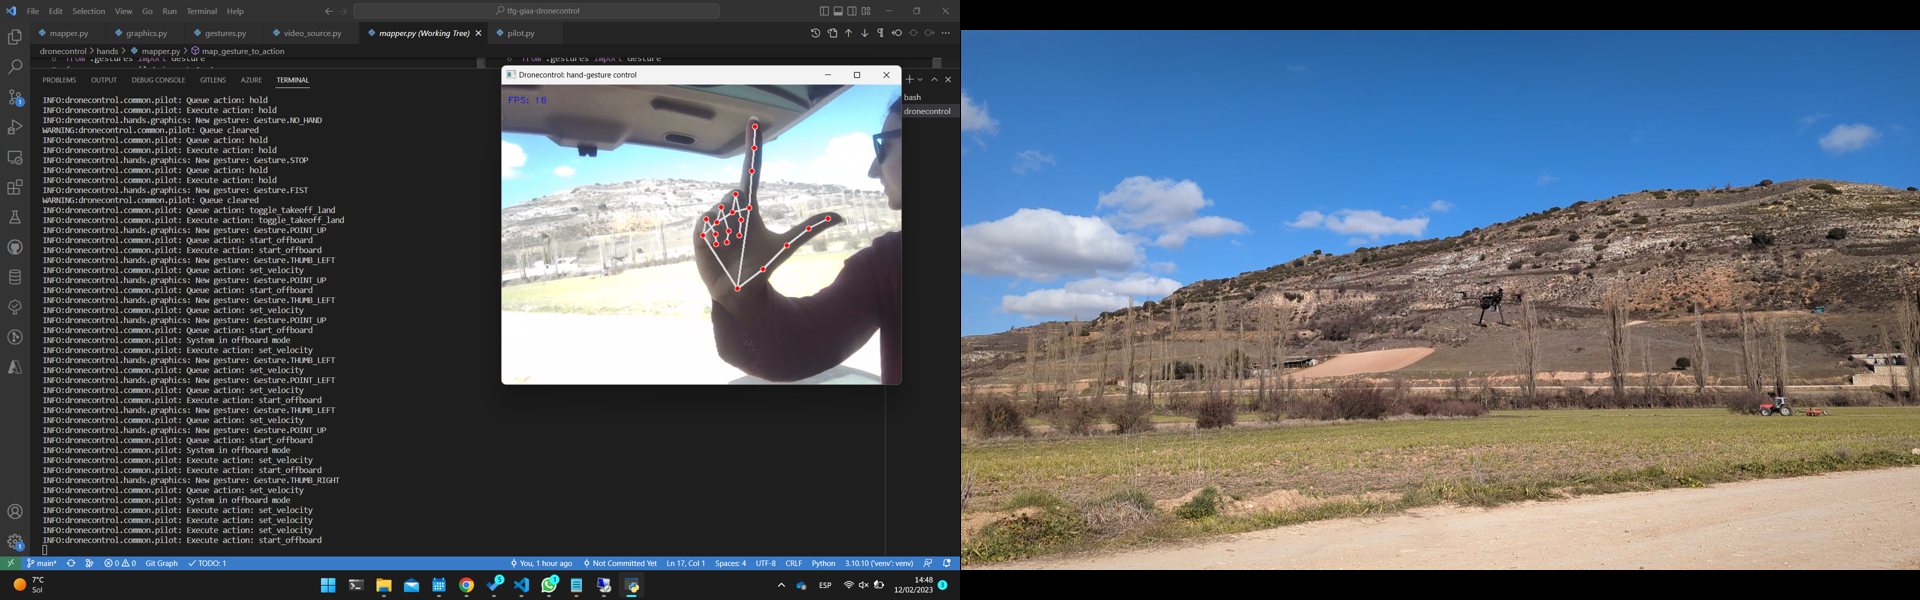
\includegraphics[width=\textwidth, keepaspectratio]{img/video-field-test-hand.png}
  \caption{Image taken during flight controlled by the hand-gesture solution. The vehicle is moving forward.}
  \label{fig:flight-test-hand}
\end{figure}


\subsection{Follow control with onboard computer.}
\label{subsec:fl-test-5}

The last test to conduct is for the follow control solution. In this section, the companion computer will run the follow program with the aim of tracking and following a moving target outside of simulation. The setup for this test will be the same as the third test flight, described in Section \ref{subsec:fl-test-3}. Without the need for a wireless telemetry connection on the DroneVisionControl side, the telemetry radio can be utilized to track the vehicle's path using the QGroundControl application on a secondary offboard computer. The control application will be started with the following command:
\begin{minted}[breaklines, fontsize=\footnotesize, baselinestretch=1]{bash}
dronevisioncontrol follow --serial /dev/serial0:921600
\end{minted}
This \href{https://l-gonz.github.io/tfg-giaa-dronecontrol/videos/flight-test-follow}{video}\footnote{\url{https://l-gonz.github.io/tfg-giaa-dronecontrol/videos/flight-test-follow}} showcases the process of the vehicle taking off (T key) and activating offboard flight mode (O key) to initiate the tracking of a detected figure. Figure \ref{fig:flight-test-follow} presents an image extracted from this video.


\begin{figure}[H]
  \centering
  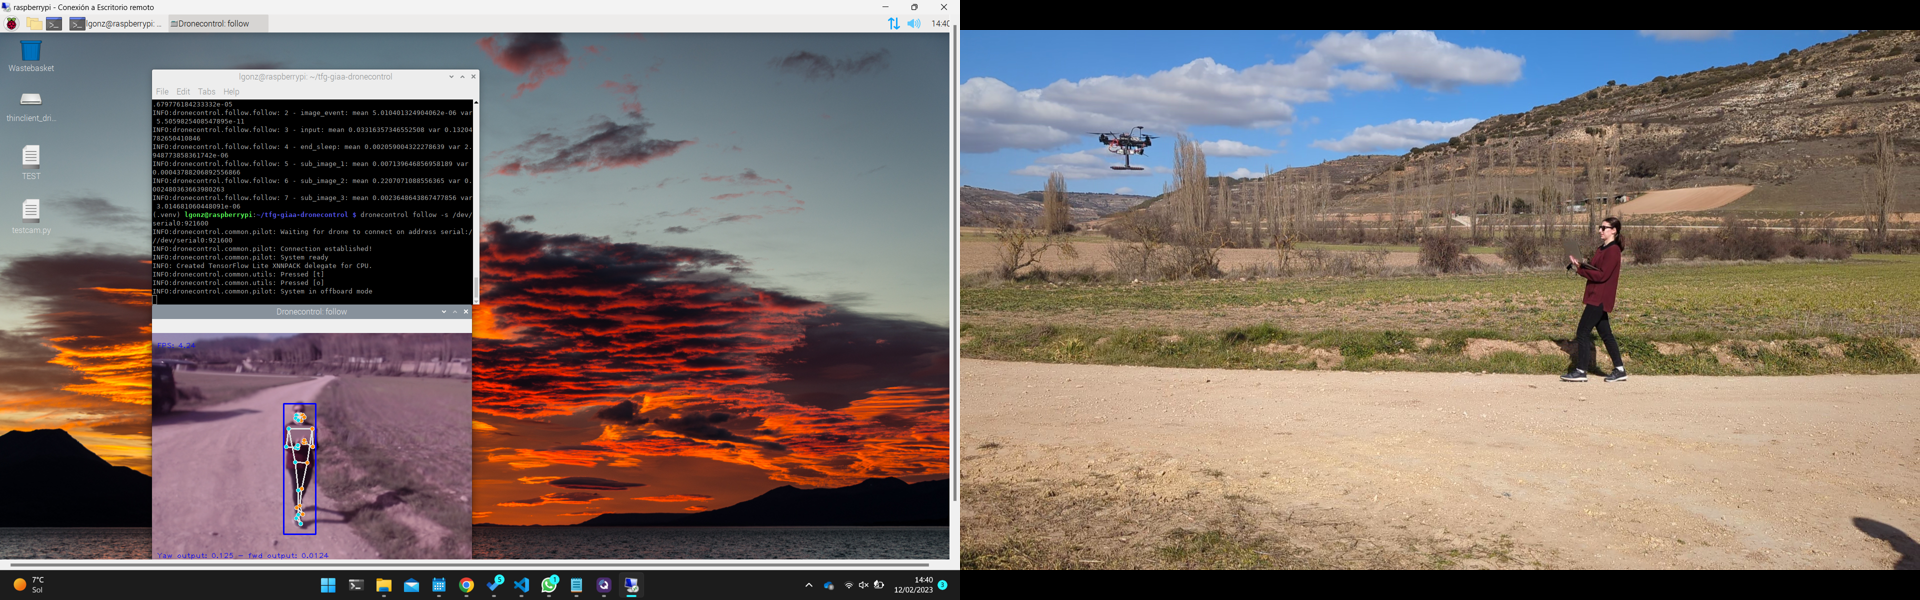
\includegraphics[width=\textwidth, keepaspectratio]{img/video-field-test-follow.png}
  \caption{Terminal and image output of the DroneVisionControl follow solution running on the Raspberry Pi.}
  \label{fig:flight-test-follow}
\end{figure}


During the flight test, the application running on the Raspberry Pi achieves a maximum frame rate of around 6 FPS when the follow mechanism is active and approximately 8 FPS when it is disabled by switching out of offboard flight mode. In practical terms, this means that the person being tracked by the drone needs to move relatively slowly to ensure that the camera does not lose sight of them before the control loop can send the command to the vehicle to move to the previously detected position. However, for a proof-of-concept scenario, this performance is acceptable.


At the end of the program execution, the average loop time and average runtime for each task in the control loop are displayed in the terminal. Based on the measurements obtained during the test flight, the average frame rate is calculated to be 3.58 FPS. Figure \ref{fig:flight-performance} compares these measurements with those analyzed in Section \ref{subsec:performance}, particularly with the test configuration selected to most closely resemble actual flight conditions (autopilot board running on HITL mode and the companion computer powered by the secondary battery). Very similar results are recorded for both tests, confirming the simulation configuration employed as a valid method of obtaining realistic results without complex or costly flight tests.

Overall, this test flight verifies the effectiveness of the follow control solution and its ability to track and follow a moving target during a real flight scenario, as well as the validity of the simulation process to obtain realistic results.


\begin{figure}
  \centering
  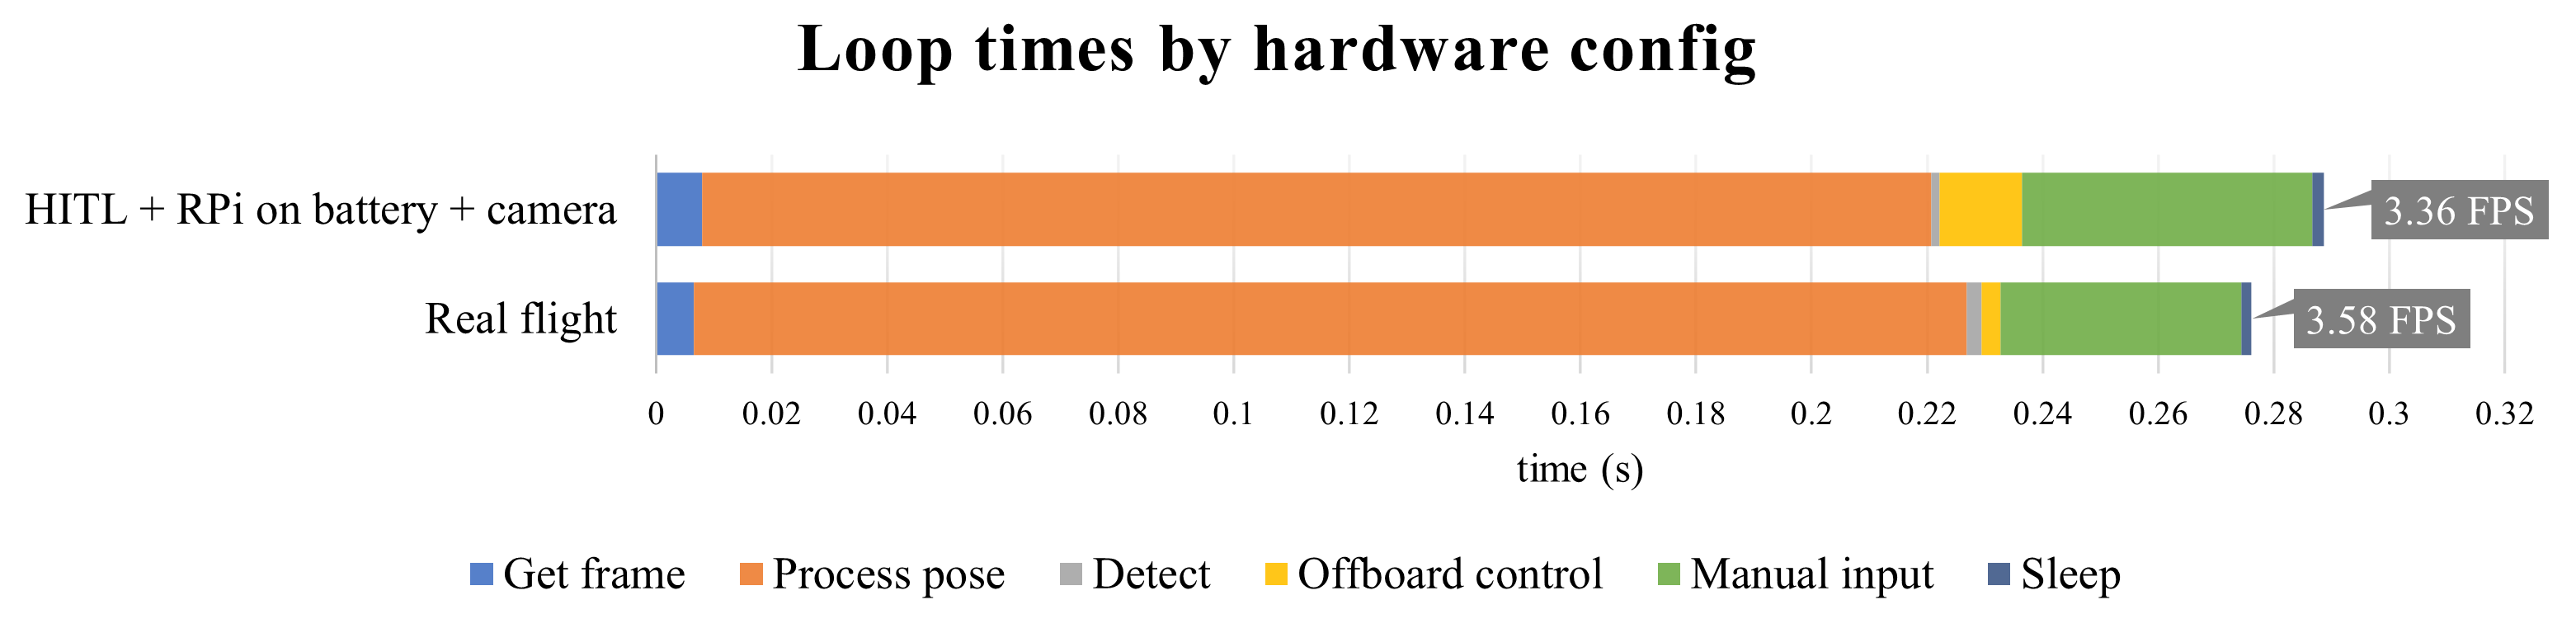
\includegraphics[width=\textwidth, keepaspectratio]{img/perf-hitl-flight.png}
  \caption{Average loop time for each individual task in the follow control solution and total frame rate for realistic simulation versus actual test flights.}
  \label{fig:flight-performance}
\end{figure}
